\documentclass[11pt, a4paper]{paper}
\usepackage{a4wide,color}

\usepackage[utf8]{inputenc}
\usepackage[T1]{fontenc}
\usepackage[frenchb]{babel}

\usepackage{graphicx}
\usepackage{amssymb}
\usepackage{hyperref}

\usepackage{amstext}
\usepackage{amsmath}


\usepackage{placeins}


\usepackage{framed}


\title{{\Huge Rapport de projet De Stijl}\\
{\large version \today}\\
---\\
}
\author{\color{black}{ABDELMOUMEN Oussama ()} \\ {GRASA Guillaume ()}\\ {HELLO Anouk ()} \\ {PROUVOST Chloé ()} \\
\color{blue}{Exemple : P.-E. Hladik (conception, robot, rédaction du compte-rendu)}
}

\begin{document}

%%%%%%%%%%%%%%
% PAGE DE GARDE
\maketitle


{\color{red}
\begin{framed}
\begin{center}{\bf\Large --- Ce qu'il faut faire --- } \end{center}

{\bf Remplacez tous les textes en bleu et supprimer les textes en rouge}\\


{\bf Le rapport est à rendre en pdf et à envoyer par mail à votre encadrant de TP au plus tard le 20 janvier 2017.}\\

{\bf Vous devez aussi rendre votre code (uniquement les fichiers que vous avez écrits ou modifiés) sous la forme d'une archive (zip ou tar).}\\

Vous pouvez utiliser word ou un autre logiciel d'édition pour rédiger ce rapport, par contre vous devez  {\bf obligatoirement} respecter la structure décrite ici.\\


Critères d'évaluation :
\begin{itemize}
	\item Qualité rédactionnelle,
	\item Exhaustivité et justesse des règles de codage,
	\item Qualité de la conception (clarté, respect de la syntaxe, exhaustivité, justesse),
	\item Qualité des explications,
	\item Respect des règles dans la production du code\\
\end{itemize}

Compétences évaluées :
\begin{itemize}
	\item rédaction et communication sur un dossier de conception
	\item concevoir une application concurrente temps réel
	\item analyser une conception
	\item passer d'un modèle de conception à une implémentation
	\item écriture de code C et utilisation de primitives au niveau système
\end{itemize}
\end{framed}
}

%%%%%%%%%%%%%%
% DEBUT DU RAPPORT
\newpage


%%%%%%%%%%%%%%
% CONCEPTION
\section{Conception}

{\color{red} Mettez dans cette partie tous les éléments de votre conception en particulier vos diagrammes AADL (vue globale du système et détails des threads). Cette partie doit être auto-suffisante pour comprendre votre application.

Pour faciliter la lecture des schémas, vous allez présenter votre conception en trois parties, l'une focalisée sur la communication entre le moniteur et le superviseur, la seconde consacrée au contrôle du robot et la troisième au traitement vidéo.

{\bf La partie de gestion automatique d'une mission du robot sera à part pour ceux l'ayant traitée.}

Si vous le souhaitez, au lieu de dessiner vos diagrammes sous un éditeur, vous pouvez joindre un scan de vos schémas — ils doivent être lisibles et propres.}

% VUE GENERAL DU SYSTEME
\subsection{Diagramme fonctionnel général}

{\color{red} Mettez ici un diagramme fonctionnel qui présente les principaux blocs de votre conception. Pour cela, inspirez vous du diagramme ci-dessous (fig.~\ref{fig:diag_fonc_gen}) en indiquant pour chaque groupe de threads les données et ports partagés. La figure~\ref{fig:diag_fonc_gen} a été réalisée à partir du document de conception. {\bf Vous devez absolument conserver le découpage en trois groupes de threads ({\tt th\_group\_gestion\_moniteur}, {\tt th\_group\_gestion\_robot}, {\tt th\_group\_vision}).}}

\begin{figure}[htbp]
\label{fig:diag_fonc_gen}
\begin{center}
{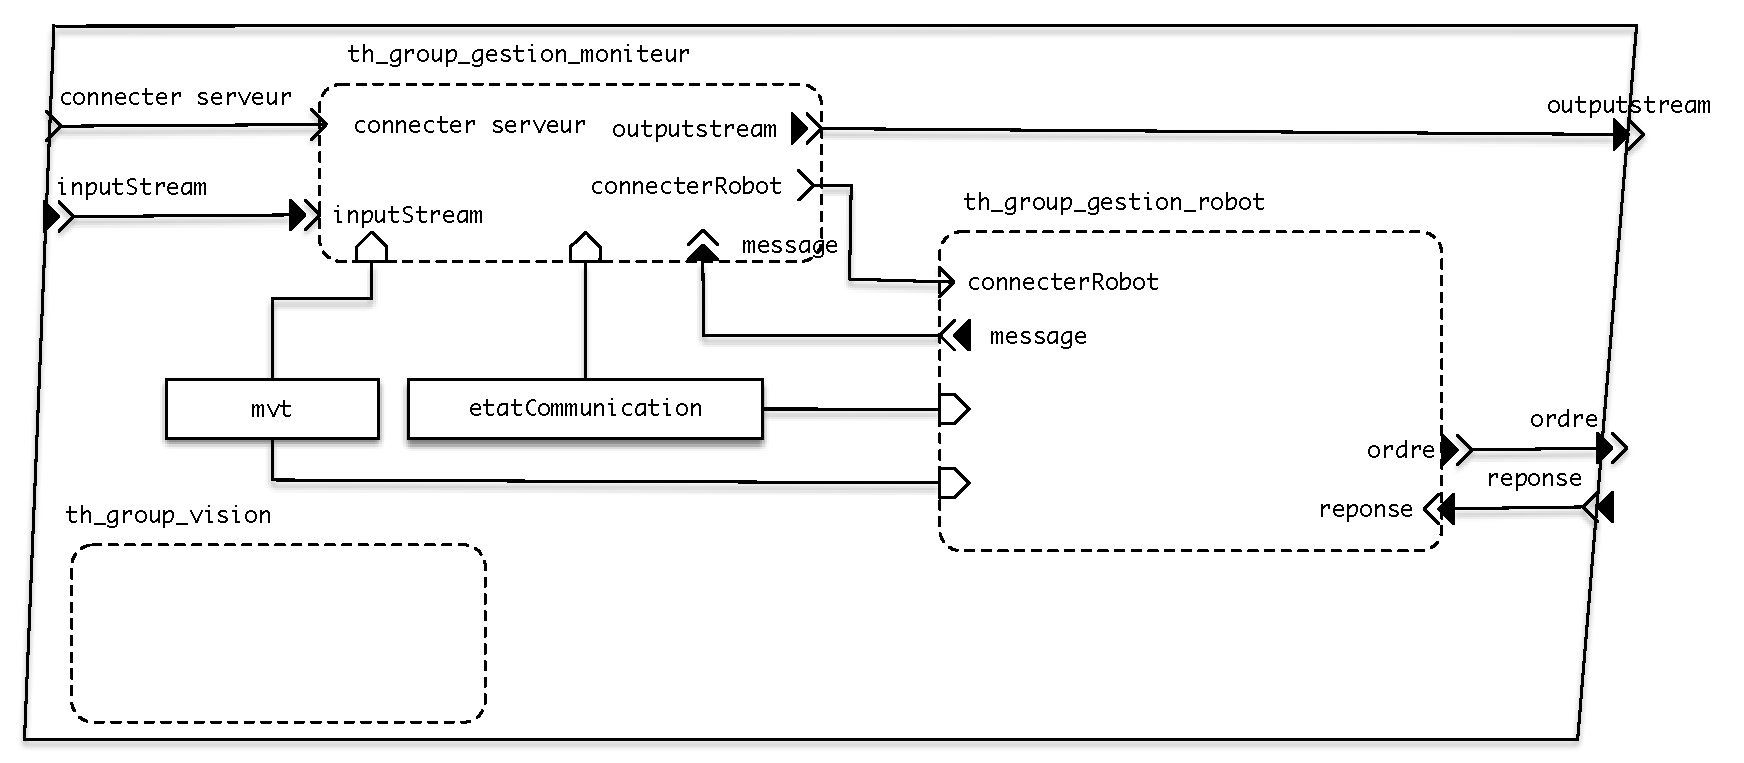
\includegraphics[scale=.5]{./figures-pdf/diag_fonc_gen}}
{\caption{Diagramme fonctionnel du système}}
\end{center}
\end{figure}
\FloatBarrier

% DIAGRAMME FONCTIONNEL GT MONITEUR
\subsection{Groupe de threads gestion du moniteur}

{\color{red}Placez ici :
\begin{itemize}
\item le diagramme fonctionnel en AADL décrivant le groupe de threads de gestion du moniteur (voir exemple de la figure~\ref{fig:diag_fonc_moniteur} réalisée à partir du dossier de conception),
\item remplir le tableau~\ref{tab:gt_moniteur} pour expliquer le rôle de chacun des threads,
\item les diagrammes d'activité de chaque thread de ce groupe.
\end{itemize}

Décrivez tous les éléments (paramètres, variables, etc.) qui vous semblent pertinents pour comprendre les diagrammes.}

% DIAGRAMME FONCTIONNEL GT MONITEUR
\subsubsection{Diagramme fonctionnel du groupe gestion du moniteur}

{\color{red} Exemple de diagramme fonctionnel pour le groupe de thread de gestion du moniteur. Mettez à jour ce diagramme avec votre conception.}

\begin{figure}[htbp]
\label{fig:diag_fonc_moniteur}
\begin{center}
{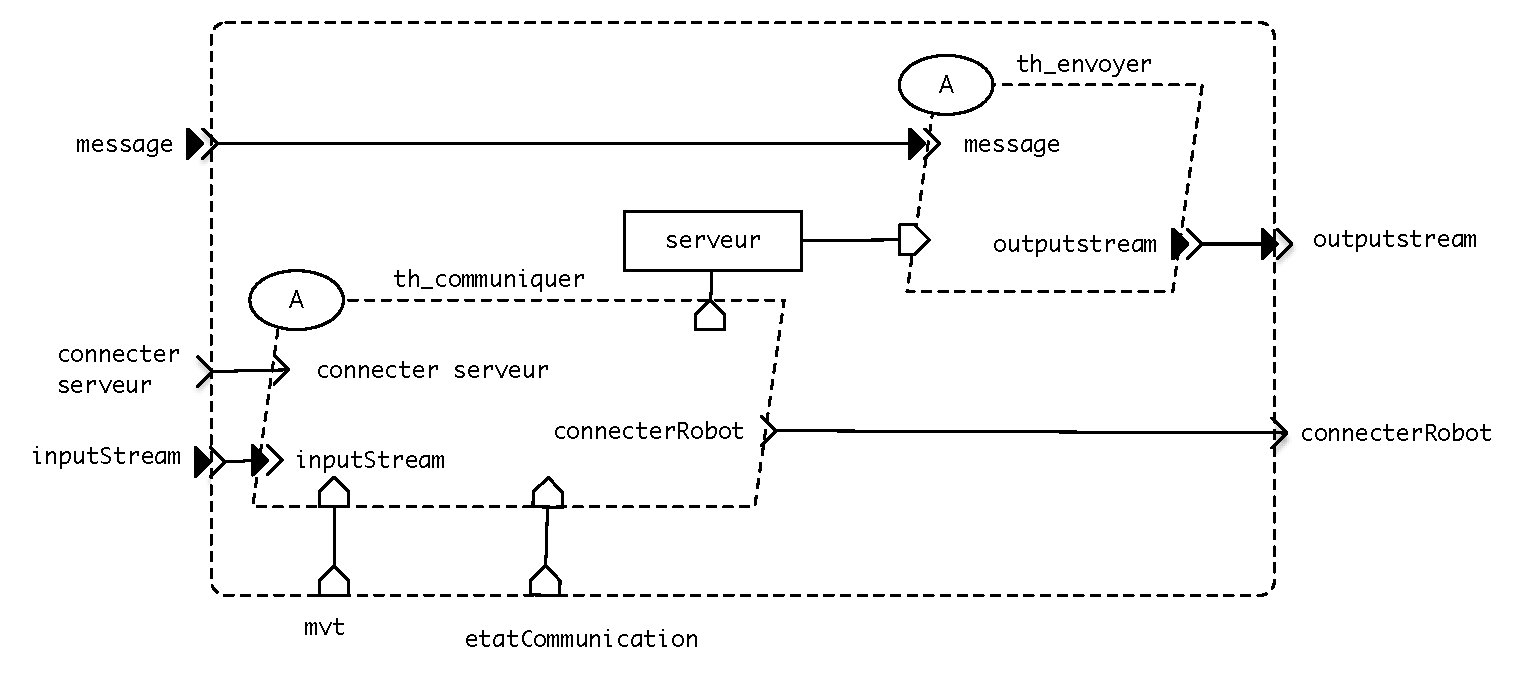
\includegraphics[scale=.5]{./figures-pdf/diag_fonc_moniteur}}
{\caption{Diagramme fonctionnel du groupe de threads gestion du moniteur}}
\end{center}
\end{figure}
\FloatBarrier

% DESCRIPTION THREADS GT MONITEUR
\subsubsection{Description des threads  du groupe gestion du moniteur}
{\color{red} Remplissez le tableau ci-dessous pour expliquer le rôle de chaque thread et donner son niveau de priorité.}


\begin{table}[htp]
\caption{Description des threads du groupe {\tt th\_group\_gestion\_moniteur}}
\begin{center}
\begin{tabular}{|p{3cm}|p{8.5cm}|p{2cm}|}
\hline
\bf Nom du thread &	\bf Rôle &	\bf Priorité \\
\hline
\hline
\color{black}thCommuniquer	& \color{black}Prend en charge les messages entrants depuis le moniteur & \color{black}25\\
\hline
\color{black}thEnvoyer	& \color{black}Envoi l'ensemble des messages du superviseur au moniteur & \color{black}30\\
\hline
\color{black}... &	\color{black}... &	\color{black}...\\
\hline
\end{tabular}
\end{center}
\label{tab:gt_moniteur}
\end{table}%

% DIAGRAMMES D'ACTIVITE GT MONITEUR
\subsubsection{Diagrammes d'activité  du groupe gestion du moniteur}
{\color{red}Décrivez le comportement de chacun de vos threads avec des diagrammes d'activité. Apportez les explications qui vous semblent nécessaires pour comprendre votre conception. A titre d'exemple les diagrammes fonctionnels tirés du document de conception sont remis.}

\begin{figure}[htbp]
\label{fig:act_communiquer}
\begin{center}
{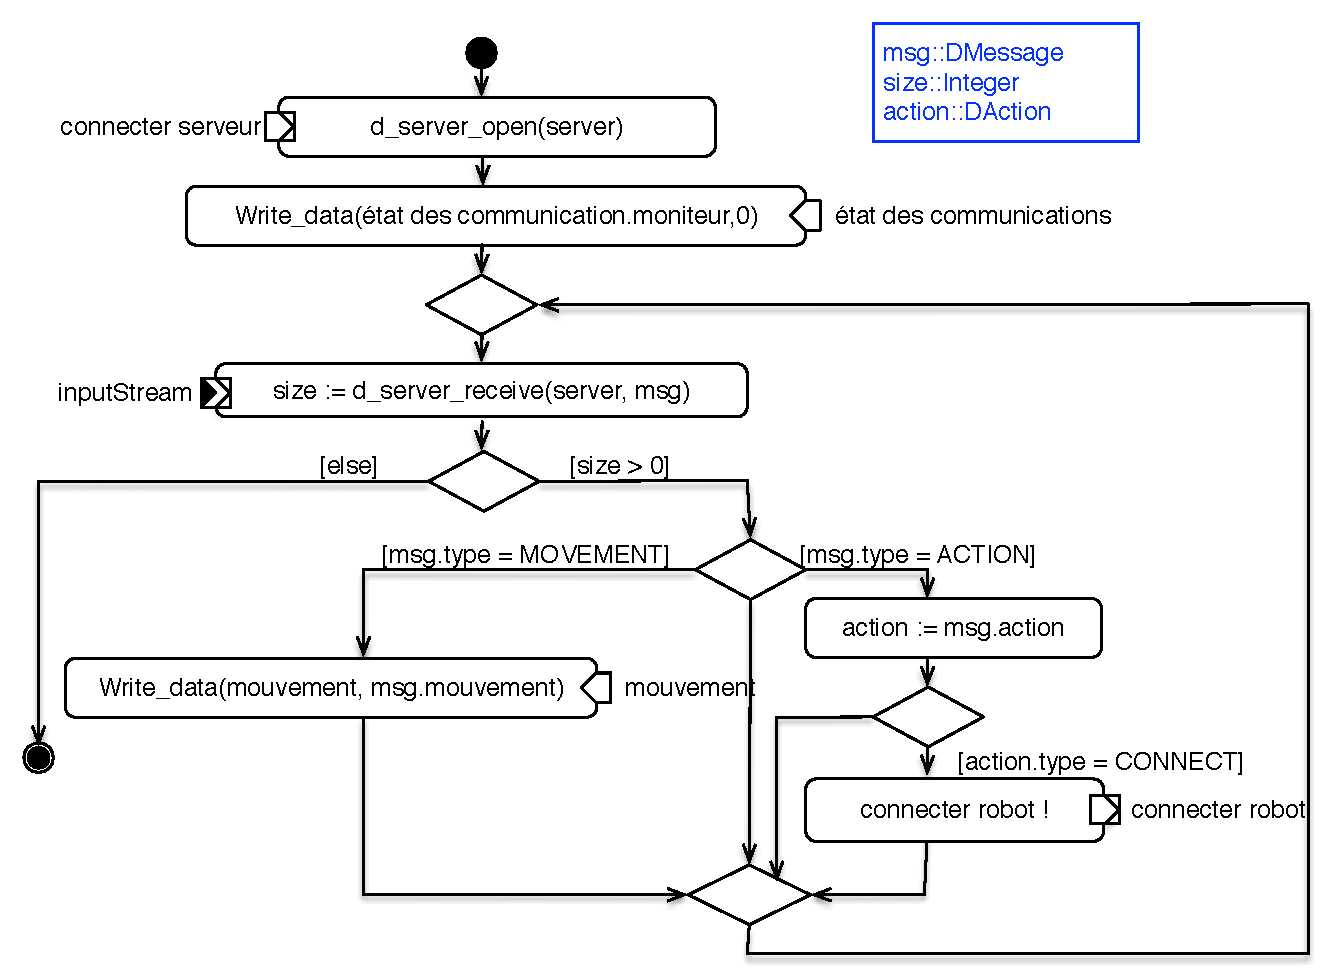
\includegraphics[scale=.5]{./figures-pdf/act_communiquer}}
{\caption{Diagramme d'activité du thread {\tt th\_communiquer}}}
\end{center}
\end{figure}
\FloatBarrier

\begin{figure}[htbp]
\label{fig:act_envoyer}
\begin{center}
{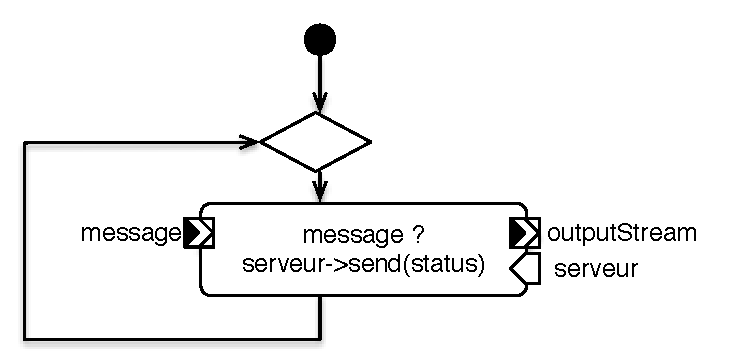
\includegraphics[scale=.5]{./figures-pdf/act_envoyer}}
{\caption{Diagramme d'activité du thread {\tt th\_envoyer}}}
\end{center}
\end{figure}
\FloatBarrier

% DIAGRAMME FONCTIONNEL GT ROBOT
\subsection{Groupe de threads gestion du robot}

% DIAGRAMME FONCTIONNEL GT ROBOT
\subsubsection{Diagramme fonctionnel du groupe gestion robot}
{\color{blue} Ajoutez le diagramme fonctionnel du groupe de threads de gestion du robot.}

% DESCRIPTION THREADS GT ROBOT
\subsubsection{Description des threads du groupe gestion robot}
{\color{red} Remplissez le tableau ci-dessous pour expliquer le rôle de chaque thread et donner son niveau de priorité.}


\begin{table}[htp]
\caption{Description des threads du groupe {\tt th\_group\_gestion\_robot}}
\begin{center}
\begin{tabular}{|p{3cm}|p{8.5cm}|p{2cm}|}
\hline
\bf Nom du thread &	\bf Rôle &	\bf Priorité \\
\hline
\hline
\color{black}thConnecter &	\color{black}Ouvre la communication avec le robot &	\color{black}...\\
\hline
\color{black}thReloadWatchdog &	\color{black}Surveille la perte de communication entre le robot et le superviseur &	\color{black}(forte priorité)\\
\hline
\color{black}thDeplacer &	\color{black}Envoi des ordres de déplacement au robot &	\color{black}...\\
\hline
\color{black}thEtatBatterie &	\color{black}Surveille l'état de la batterie du robot et l'envoi au moniteur via le thread thEnvoyer &	\color{black}...\\
\hline
\end{tabular}
\end{center}
\label{tab:gt_moniteur}
\end{table}%
\FloatBarrier

% DIAGRAMMES D'ACTIVITE GT ROBOT
\subsubsection{Diagrammes d'activité du groupe robot}
{\color{blue}Décrivez le comportement de chacun de vos threads avec des diagrammes d'activité. Apportez les explications qui vous semblent nécessaires pour comprendre votre conception.}

% DIAGRAMME FONCTIONNEL GT VISION
\subsection{Groupe de threads vision}

% DIAGRAMME FONCTIONNEL GT VISION
\subsubsection{Diagramme fonctionnel du groupe vision}

{\color{blue} Ajoutez le diagramme fonctionnel du groupe de threads de vision.}

% DESCRIPTION THREADS GT VISION
\subsubsection{Description des threads du groupe vision}
{\color{red} Remplissez le tableau ci-dessous pour expliquer le rôle de chaque thread et donner son niveau de priorité.}


\begin{table}[htp]
\caption{Description des threads du groupe {\tt th\_group\_vision}}
\begin{center}
\begin{tabular}{|p{3cm}|p{8.5cm}|p{2cm}|}
\hline
\bf Nom du thread &	\bf Rôle &	\bf Priorité \\
\hline
\hline
\color{black}thTraitementImage &	\color{black}Capture une image, si l'utilisateur souhaite la position du robot, il la dessine sur cette image, compresse l'image et l'envoi en message. Si il ne veux pas la position il compresse l'image puis l'envoi en message. Il ne peut pas s'exécuter si il y a une calibration. &	\color{blue}...\\
\hline
\color{black}thCalibration &	\color{black}Détection de l'arène, l'utilisateur doit valider la calibration ou redemander une détection &	\color{blue}...\\
\hline
\end{tabular}
\end{center}
\label{tab:gt_moniteur}
\end{table}%
\FloatBarrier

% DIAGRAMMES D'ACTIVITE GT VISION
\subsubsection{Diagrammes d'activité du groupe vision}
{\color{blue}Décrivez le comportement de chacun de vos threads avec des diagrammes d'activité. Apportez les explications qui vous semblent nécessaires pour comprendre votre conception.}




%%%%%%%%%%%%%%%
% ANALYSE ET VALIDATION
\section{Analyse et validation de la conception}

{\color{red}
Pour les trois exigences suivantes montrer en quoi votre conception permet d’y répondre. }

% EXIGENCE EXEMPLE
{\color{red} \subsection*{Exemple de ce qui est attendu}

Voici un exemple avec pour exigence : \og une fois la communication établie avec le robot, les ordre de mouvement sélectionnés par l'utilisateur sur le moniteur sont transmis au robot.\fg\ 

Il faut justifier à travers la conception que cette exigence est bien prise en considération et estimer le temps maximum que peut prendre la transmission d'un ordre.

Pour illustrer cela, je m'appuie sur la première conception du système qui est faite  dans le document \og Dossier de conception \fg.

{\bf Justification} : une fois la communication établie, les ordres de l'utilisateur sont reçus par le superviseur via le port {\tt connecter\_serveur} du thread {\tt th\_communiquer} (attente de la fonction {\tt d\_server\_receive} sur la figure 4).

Le diagramme d'activité du thread (fig. 4) montre qu'à la réception d'un message de type MOUVEMENT la valeur qu'il porte est écrite dans la donnée partagée {\tt mouvement}. 

Cette donnée est lue périodiquement par le thread {\tt th\_deplacer}. Son diagramme d'activité (fig. 7) montre qu'en fonction de la valeur de la donnée {\tt mouvement} les variables  internes à {\tt th\_deplacer} nommées {\tt gauche} et {\tt droite} sont mises à jour pour ensuite être transmises au robot via l'appel à la fonction {\tt d\_robot\_set\_motor}.

{\bf Estimation du temps de traitement} : la figure~\ref{fig:seq} montre la séquence d'exécution la plus désavantageuse pour la prise en compte d'un ordre de mouvement. L'utilisateur commence par sélectionner son ordre sur l'interface graphique qui ajoute un délai de 200~ms avant de le transmettre au superviseur (on ignore ici les délais réseaux). Le thread {\tt th\_communiquer} étant le plus prioritaire, il traite immédiatement le message (on remarque par exemple sur la figure la préemption du thread {\tt th\_deplacer}). Le temps de traitement de {\tt th\_communiquer} est estimer à 1~ms d'après le document \og Dossier de conception \fg.

La pire des situations est une exécution du thread {\tt th\_deplacer} juste avant la réception du message de mouvement qui devra attendre 1 seconde avant de lire la nouvelle valeur de {\tt mouvement}. Le temps de transmission de l'ordre au robot a été estimé à 41~ms (voir p.~12 du document \og Dossier de conception \fg).

Nous avons donc un délai possible de l'ordre de 0.2+0.001+1+0.041 = 1.242~s entre la sélection d'un mouvement par l'utilisateur et sa réception par le robot.

\begin{figure}[htbp]
\begin{center}
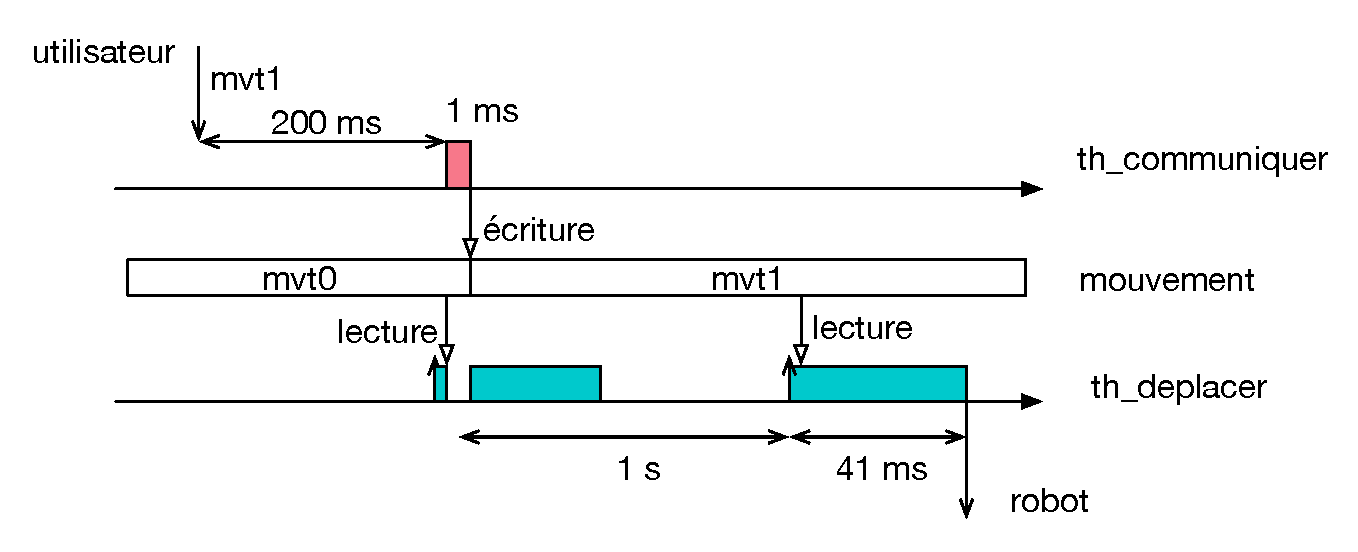
\includegraphics[scale=0.6]{./figures-pdf/sequence}
\caption{\color{red}Exemple de pire séquence d'exécution pour la transmission d'un ordre de mouvement au robot.}
\label{fig:seq}
\end{center}
\end{figure}
}

% EXIGENCE 1
\subsection{Exigence 1 : En cas de perte de communication entre le robot et le superviseur, le robot est stoppé et le nouvel état est signalé à l'utilisateur via le moniteur.}

{\color{blue} Expliquez en vous appuyant sur votre conception comment vous garantissez que cette exigence est toujours respectée.}
{\color{black} Watchdog + Compteur (variable globale)}

{\color{blue} Fournissez un chronogramme (ou un diagramme de séquence si vous préférez) avec l’ordonnancement de votre système et estimer la plus grande durée entre l'instant où la communication est perdue et l'instant où l'utilisateur en est informé.}

% EXIGENCE 2
\subsection{Exigence 2 : La communication entre le robot et le superviseur est déclarée perdue si et seulement si trois échecs successifs de communication entre le robot et le superviseur surviennent.}

{\color{blue} Expliquez en vous appuyant sur votre conception comment vous pouvez garantir que cette exigence est toujours respectée.\\}
{\color{black} Grace au compteur qui est une variable partagée enter les threads qui communiquent avec le robot. Il est incrémenté à chaque fois que le robot ne répond pas à une requête. Lorsqu'il atteint 3, on envoie un message au moniteur pour en informer l'utilisateur.}

% EXIGENCE 3
\subsection{Exigence 3 : 
L'image qui est  affichée sur le moniteur ne doit pas être plus vieille que 600~ms (différence de temps entre la capture de l'image et son affichage sur le moniteur).}

{\color{blue} Expliquez en vous appuyant sur votre conception comment vous garantissez que cette exigence est toujours respectée. \\}
{\color{black} thread traitement image, periode 600ms. Il a une petite priorité. 4*40ms + 250ms < 600 ms \\}
{\color{blue} Fournissez un chronogramme (ou un diagramme de séquence si vous préférez) avec l’ordonnancement de votre système qui montre en quoi cela répond bien à cette exigence. Expliquez.}


%%%%%%%%%%%%%%%%%%%
% TRANSFORMATION AADL2XENO
\section{Transformation AADL2XENO}
 
 {\color{red} Cette section est consacrée aux moyens pour passer d'un modèle AADL au code. Pour chacun des éléments AADL, vous allez expliquer {\bf comment le traduire en C} et quels {\bf services de Xenomai} vous avez utilisés {\bf en expliquant ce qu'il fait}. N'hésitez pas à illustrer avec des extraits de code.}
 
% THREAD
\subsection{Thread}
% INSTANCIATION THREAD
\subsubsection{Instanciation et démarrage}
 {\color{blue} Expliquer comment vous implémentez sous Xenomai l'instanciation et le démarrage d'un  thread AADL.}
 
{\color{blue} {\bf Exemple de réponse} : Un thread AADL est instancié en C par une tâche ({\tt RT\_TASK}) Xenomai.  Pour cela, une structure {\tt RT\_TASK} est déclarée comme variable globale pour chaque tâche.

Le service {\tt rt\_task\_create} est utilisé pour créer la tâche, c'est-à-dire réserver son space mémoire et la déclarer au noyau, et {\tt rt\_task\_start} pour lancer l'exécution de la tâche.}

% CODE THREAD
\subsubsection{Code à exécuter}
 {\color{blue} Comment se fait le lien sous Xenomai entre le thread et le traitement à exécuter.}

% PRIORITE THREAD
\subsubsection{Niveau de priorités}
 {\color{blue} Expliquer comment vous fixez sous Xenomai le niveau de priorité d'un thread AADL.}

% PERIODICITE THREAD
\subsubsection{Activation périodique}
 {\color{blue} Expliquer comment vous rendez périodique l'activation d'un thread AADL sous Xenomai.}

% THREAD EVENEMENTIEL
\subsubsection{Activation événementielle}
 {\color{blue} Expliquer les moyens mis en {\oe}uvre dans l'implémentation sous Xenomai pour gérer les activations événementielles d'un thread AADL.}

% PORT D'EVENEMENT
\subsection{Port d’événement}

% INSTANCIATION PORT D'EVENEMENT
\subsubsection{Instanciation}
 {\color{blue} Comment avez-vous instancié un port d'événement ?}

% ENVOI PORT D'EVENEMENT
\subsubsection{Envoi d’un événement}
 {\color{blue} Quels services ont été employés pour envoyer un événement ?}

% RECEPTION PORT D'EVENEMENT
\subsubsection{Réception d’un événement}
 {\color{blue} Comment se fait la synchronisation sur événement ?}

% DONNEE PARTAGEE
\subsection{Donnée partagée}

% INSTANCIATION DONNEE PARTAGEE
\subsubsection{Instanciation}
 {\color{blue} Quelle structure instancie une donnée partagée ?}

% LECTURE/ECRITURE DONNEE PARTAGEE
\subsubsection{Accès en lecture et écriture}
 {\color{blue} Comment garantissez-vous sous Xenomai l'accès à une donnée partagéé ? \\}
 {\color{black} Utilisation de mutex avec RT\_MUTEX}

% PORT D'EVENEMENT-DONNEES
\subsection{Ports d’événement-données}

% INSTANCIATION PORT D'EVENEMENT-DONNEES
\subsubsection{Instanciation}
 {\color{blue} Donnez la solution retenue pour implémenter un port d'événement-données avec Xenomai.}

% ENVOI PORT D'EVENEMENT-DONNEES
\subsubsection{Envoi d’une donnée}
 {\color{blue} Quels services avez-vous employés pour envoyer des données ?}

% RECEPTION PORT D'EVENEMENT-DONNEES
\subsubsection{Réception d’une donnée}
 {\color{blue} Quels services avez-vous employé pour recevoir des données ?}

%%%%%%%%%%%%%%%%%%%%
% EXEMPLE DE TRANSFORMATION
\section{Application de la transformation AADL2Xenomai}

{\color{blue} Vous trouverez à la fin de ce document (voir annexe~\ref{ann:conception}) une application très simple modélisée en AADL. Mettez ici le code de cette application en suivant scrupuleusement vos règles.

Ne mettez pas vos fichiers d'en-tête (sauf des extraits importants si nécessaire) et structurer le plus simplement le code. L'important est de montrer la cohérence entre les règles énoncées ci-dessus et le code que vous produisez sur l'exemple.}



%%%%%%%%%%%%%%
% EXEMPLE A TRADUIRE
\newpage
\appendix
{\color{red}
\begin{framed}
\begin{center}{\bf\Large Supprimer la partie suivante du rapport final } \end{center}
\end{framed}
}

\section{Cas d'étude à traduire}
\label{ann:conception}

L'application est un démonstration réalisée par Texas Instrument pour son système DaVinci. Ce système est dédié aux applications multimédia (vidéo, audio, etc.) et est fourni avec un BSP basé sur Linux. Il équipe des audiophones, des systèmes de surveillance, des équipements médicaux, etc.

Le diagramme~\ref{fig:vue_gen} représente le système DaVinci et l'ensemble des éléments avec lesquels il est connecté.

\begin{figure}[htp]
\begin{center}
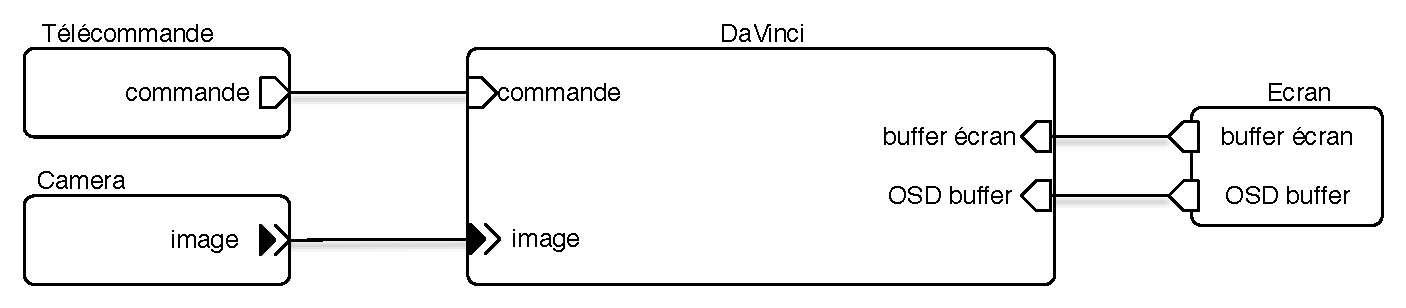
\includegraphics[scale=.6]{figures-pdf/contexte.pdf}
\caption{Vue générale du système}
\label{fig:vue_gen}
\end{center}
\end{figure}


Les différents éléments du diagramme sont :
\begin{itemize}
\item Une télécommande infrarouge qui écrit dans la zone mémoire tampon {\tt commande} les commandes émises. Cette zone est accessible en lecture depuis l'application.
\item Une caméra qui produit des données et un signal {\tt image} quand une image est disponible.
\item Un écran pour afficher les images capturées et les informations sur le système. L'affichage est mis à jour en écrivant dans le buffer de l'écran ({\tt buffer écran}). Les données contenues dans {\tt OSD buffer} sont des informations permettant d'afficher les menus à l'écran.
\end{itemize}

\subsection{Description de l'application de démonstration}

Le diagramme~\ref{fig:diag_fonc} fournit la description de l'application de démonstration de décodage vidéo de Texas Instrument.

\begin{figure}[htbp]
\begin{center}
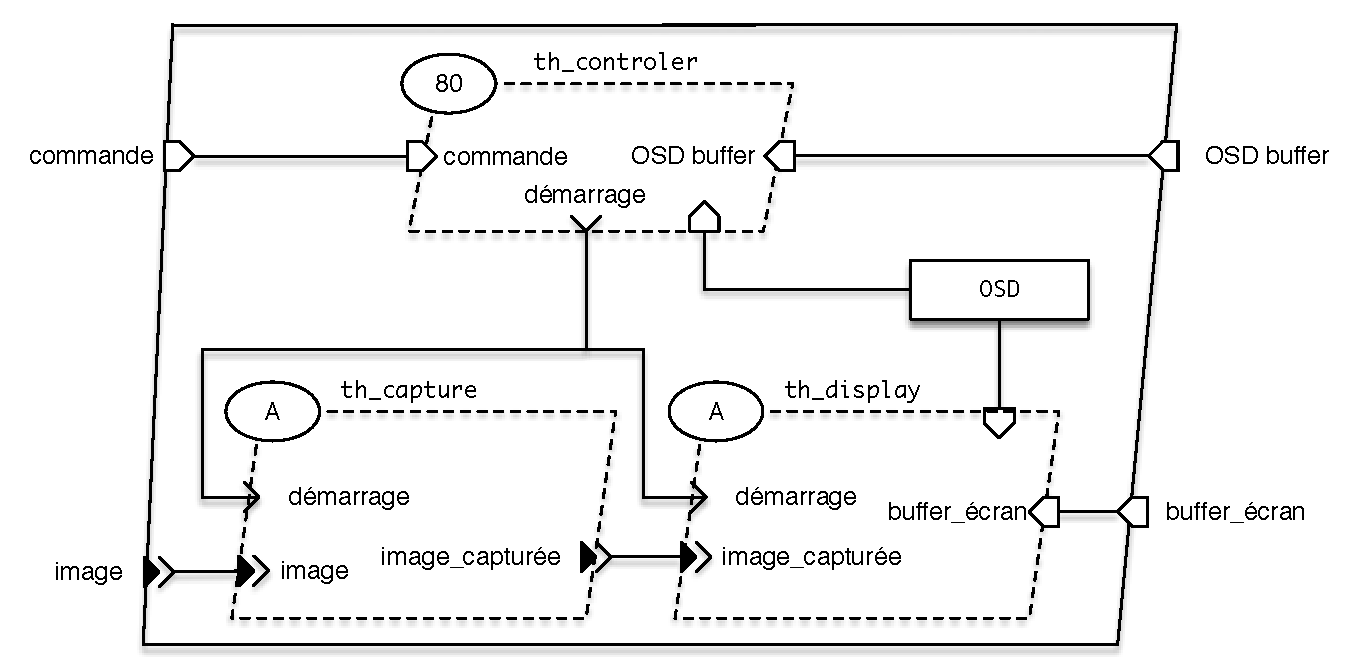
\includegraphics[scale=.45]{./figures-pdf/diag_fonc.pdf}
\caption{Diagramme fonctionnel de l'application}
\label{fig:diag_fonc}
\end{center}
\end{figure}
\FloatBarrier

\subsubsection{Description du thread th\_controler}

Le thread {\tt th\_controler} (figure~\ref{fig:th_controler}) initialise le système, synchronise toutes les tâches, puis lit les informations en provenance de la télécommande et met à jour le menu sur l'écran ainsi que les données de configuration représentées par {\tt OSD}.\\
Pour cela deux fonctions sont utilisées : {\tt initialiser\_le\_système} et {\tt calcul\_osd}.

\begin{figure}[htbp]
\label{fig:th_controler}
\begin{center}
\parbox{9cm}{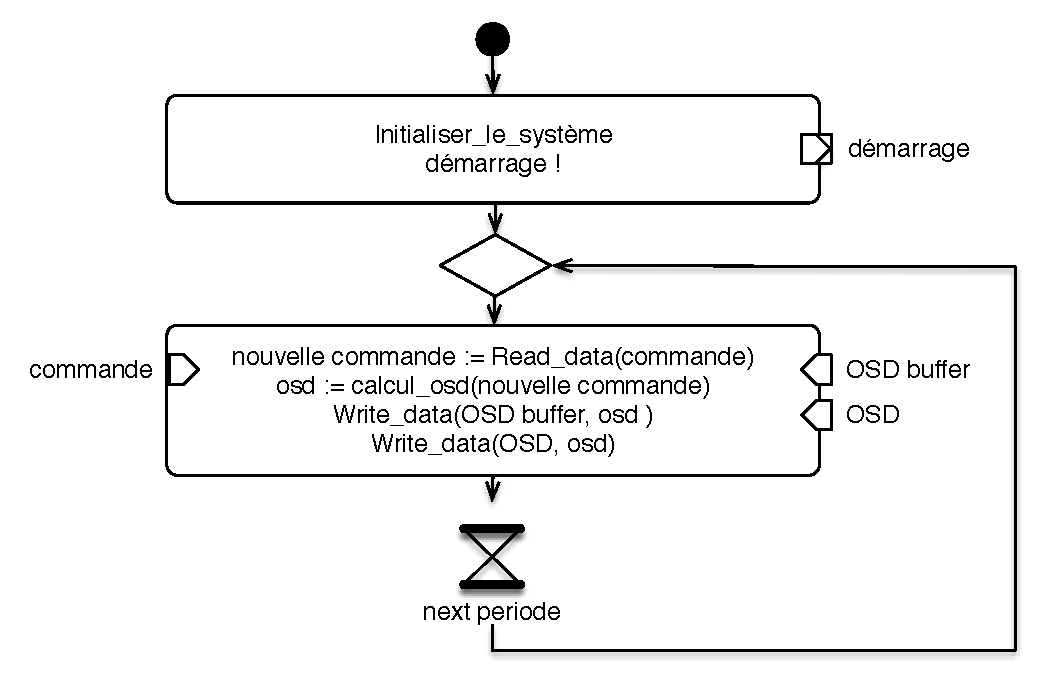
\includegraphics[scale=.5]{./figures-pdf/th_controler.pdf}}\parbox{5cm}{\caption{Diagramme d'activité du thread th\_controler}}
\end{center}
\end{figure}
\FloatBarrier


\subsubsection{Description du thread th\_capture}

Le thread {\tt th\_capture} (figure~\ref{fig:th_capture}) fait l'acquisition d'une image quand elle est disponible et la met dans une file de message.\\
La fonction {\tt acquistion\_image} est une fonction bloquante sur le port {\tt image} et retourne la valeur du port quand l'évènement se produit. En conséquence, vous n'avez pas à utiliser de service pour gérer le port de donnée-événement {\tt image}, la fonction {\tt acquistion\_image} fait le travail.

\begin{figure}[htbp]
\label{fig:th_capture}
\begin{center}
\parbox{9cm}{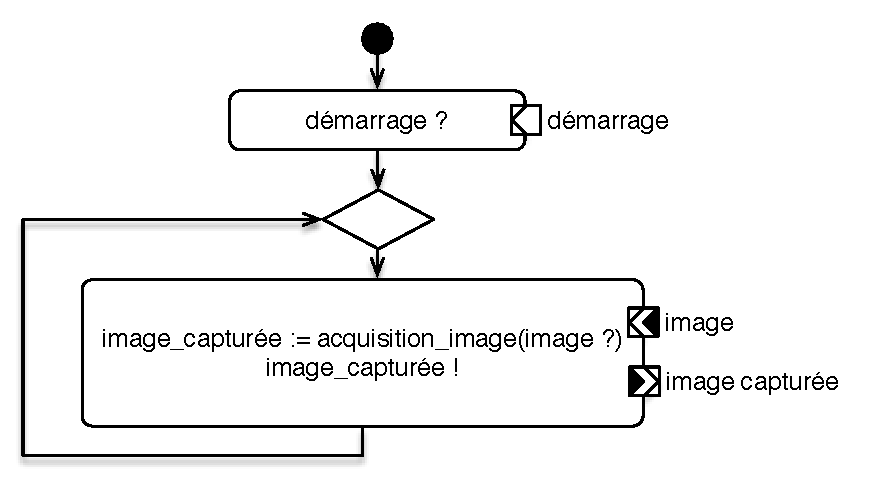
\includegraphics[scale=.5]{./figures-pdf/th_capture.pdf}}\parbox{5cm}{\caption{Diagramme d'activité du thread th\_capture}}
\end{center}
\end{figure}
\FloatBarrier

\subsubsection{Description du thread th\_display}

Le thread th\_display (figure~\ref{fig:th_display}) met à jour le buffer de l'écran en fonction des paramètres contenu dans la données OSD. Pour cela la fonction {\tt encode} est utilisée.

\begin{figure}[htbp]
\label{fig:th_display}
\begin{center}
\parbox{9cm}{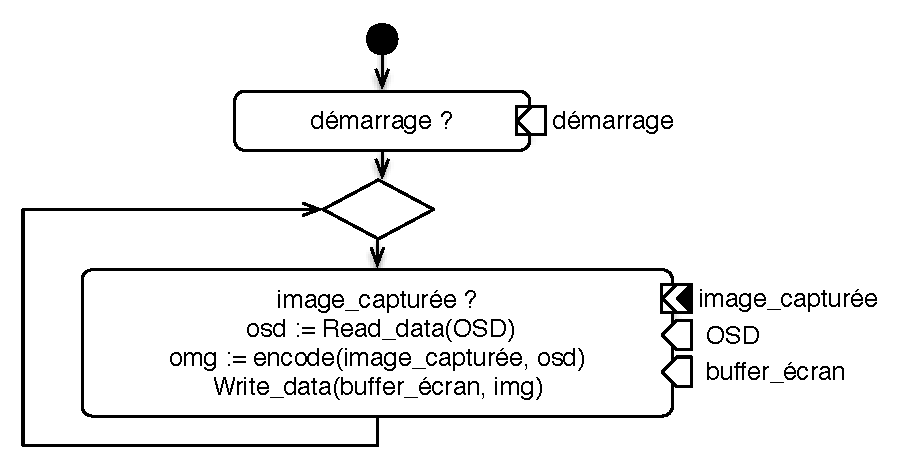
\includegraphics[scale=.5]{./figures-pdf/th_video.pdf}}\parbox{5cm}{\caption{Diagramme d'activité du thread th\_display}}
\end{center}
\end{figure}
\FloatBarrier

\subsection{Priorités}

Les priorités des threads sont fixées (plus la priorité est élevée plus la tâche est prioritaire) :

\begin{table}[ht]
\begin{center}
\begin{tabular}{|c|c|}
\hline
Thread & Priorité \\
\hline
{\tt th\_controler} & 60\\
\hline
{\tt th\_capture} & 80\\
\hline
{\tt th\_display} & 70\\
\hline
\end{tabular}
\end{center}
\end{table}%\\


\end{document}